\label{GL}

In this chapter, we will illustrate some types of guidance laws. We will be in the side of the Attacker, trying to hit the target. There is three main types of guidance laws:

% ===================================================
\section{Proportional Navigation}
% ===================================================
In this section, we will illustrate some fundamentals of missile guidance, focusing on the proportional navigation technique, which is one of the simplest guidance laws.

\subsection*{What is proportional navigation?}
The proportional navigation guidance law issues acceleration commands,
perpendicular to the instantaneous missile-target line-of-sight, which are
proportional to the line-of-sight rate and closing velocity. Mathematically, the
guidance law can be stated as

\begin{equation}
n_c= N' V_c \dot{\lambda}
\label{PNeq}
\end{equation}

where $n_c$ is the acceleration command (for the missile) in $(m/s^2)$, $N'$ is the the effective navigation ratio, a unit-less designer-chosen gain (usually in the range of $3 \to 5$), $V_c$ is the missile-target closing velocity in $(m/s)$ and $\dot{\lambda} = \frac{d\lambda}{dt}$ is the rate of the line-of-sight angle and is in $(rad/s)$. Note that (\ref{PNeq}) is dimensionally homogeneous, since $n_c$ has the dimension
\begin{equation}
\begin{split}
[n_c] &= [N'] [V_c] [\dot{\lambda}]\\
&=(1) (LT^-1) (T^-1)\\
&=LT^-2
\end{split}
\label{PN dimensionallity}
\end{equation}
which is the appropriate dimension of linear acceleration.

\subsection{Simulation of proportional navigation equations in 2-D}
\label{PNeqations}
In this subsection we will introduce the equations of proportional navigation and the sequence to get a simulation for the path of the Target and the Attacker and how the missile acceleration will be affected during this simulation.

\textbf{The simulation inputs} are the initial location of the Missile ($R_{M1}, R_{M2}$) and the initial location of the Target ($R_{T1}, R_{T2}$), Target speed $V_T$, Missile speed $V_M$, and effective navigation ratio $N'$.

There are two types of \textbf{error sources} that cause the Attacker to miss the Target; they are the heading error ($HE$) and the acceleration of the Target ($n_T$) called the Target maneuver.

\begin{figure}[htb]
	\centering
	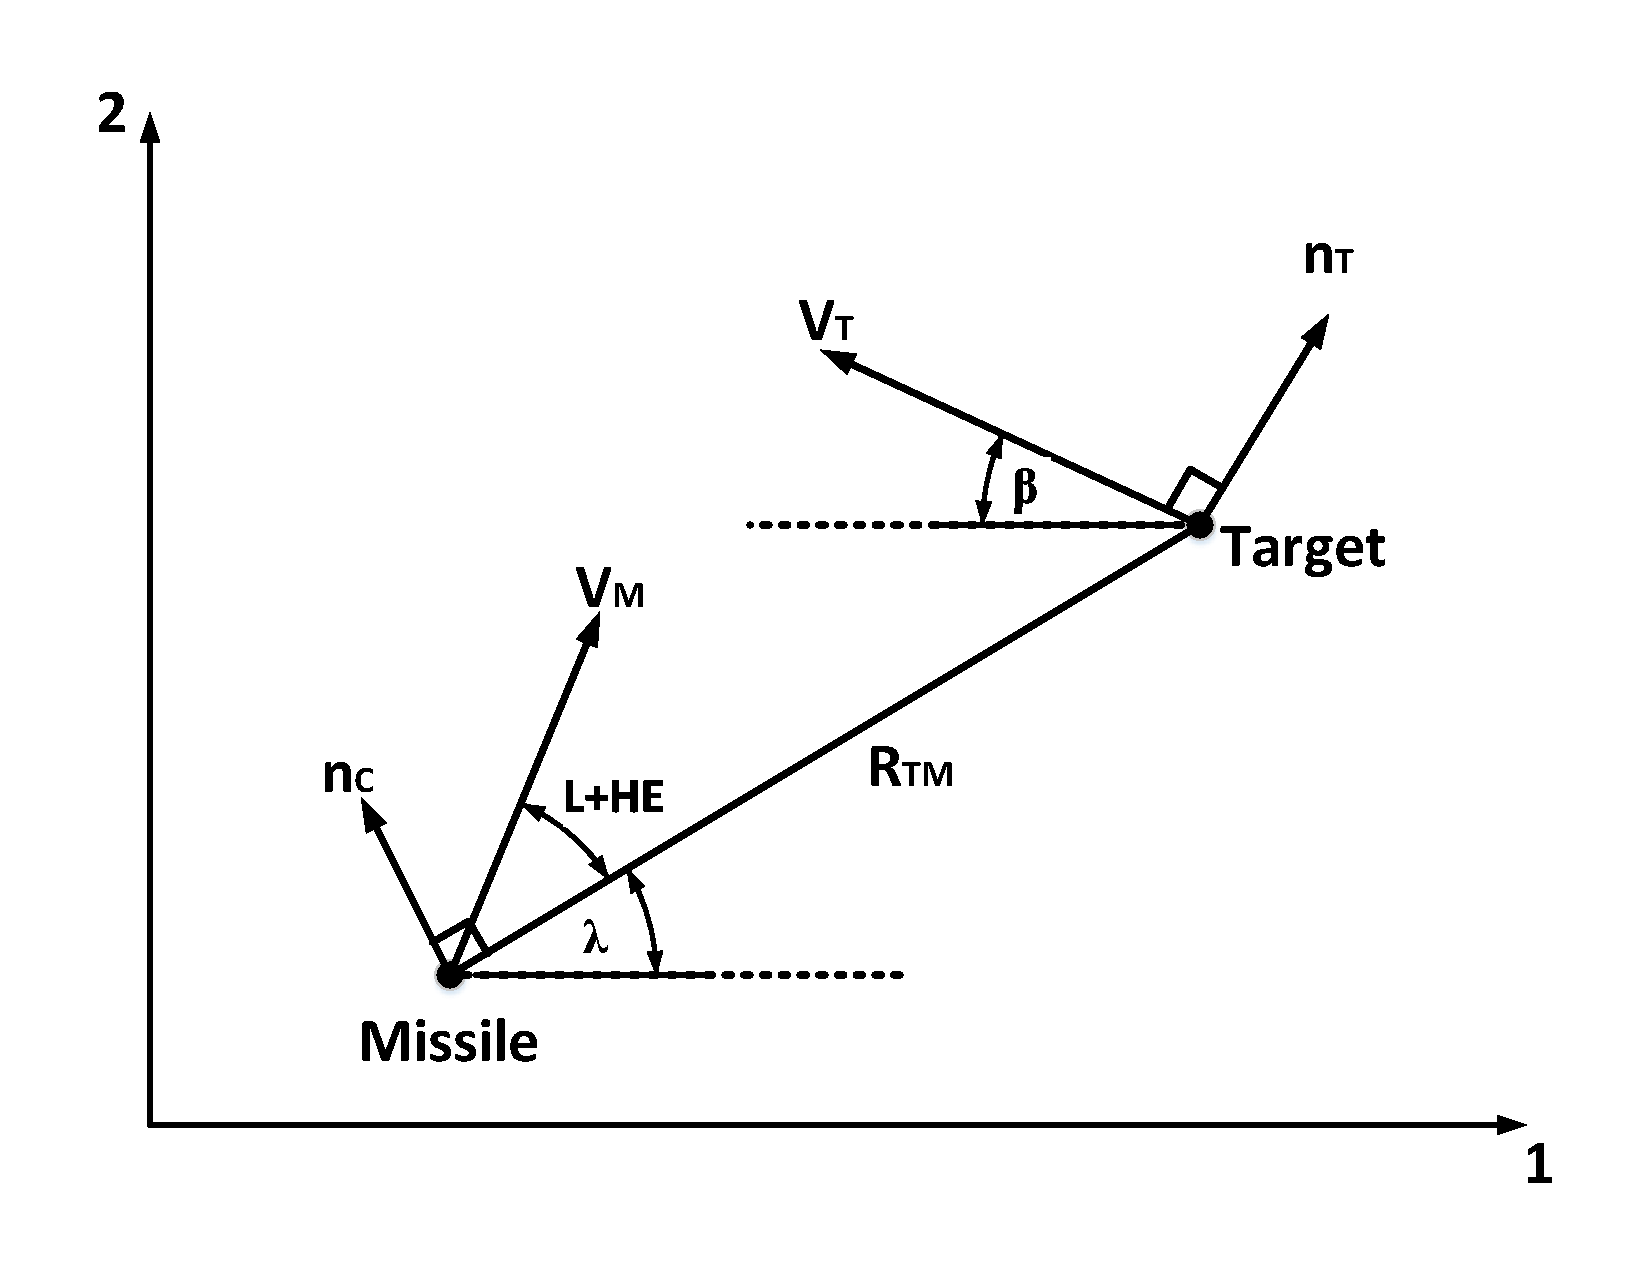
\includegraphics[scale = 0.65]{fig/PN.pdf}
	\caption{Two dimensional Missile-Target engagement geometry.}
	\label{PN}
\end{figure}


\subsubsection*{proportional navigation differential equations}

\textbf{The components of Target velocity} 
\begin{equation}
V_{T1} = - V_T \cos(\beta)
\end{equation}

\begin{equation}
V_{T2} =  V_T \sin(\beta)
\end{equation}

\textbf{Relative missile-target separation}
\begin{equation}
R_{TM1} = R{T1} - R_{M1}
\end{equation}
\begin{equation}
R_{TM2} = R{T2} - R_{M2}
\end{equation}

from the previous 2 equations we get
\begin{equation}
R_{TM} = \sqrt{R_{TM1}^2 + R_{TM2}^2}
\label{RTM}
\end{equation}

\textbf{line of sight angle}
\begin{equation}
\lambda = \tan^{-1} (\dfrac{R_{TM2}}{R_{TM1}})
\label{lambda}
\end{equation}

\textbf{missile lead angle} 
\begin{equation}
L= \sin^{-1}(\dfrac{V_T \sin(\beta + \lambda)}{V_M})
\end{equation}

the angle between the downrange axis and $V_M$ vector is $\theta = \lambda + L$

\textbf{Missile velocity components} 

\begin{equation}
V_{M1} = V_M \cos (\theta + HE)
\end{equation}

\begin{equation}
V_{M2} = V_M \sin (\theta + HE)
\end{equation}

\textbf{Relative velocity components}
\begin{equation}
V_{TM1} = V_{T1} - V_{M1}
\end{equation}

\begin{equation}
V_{TM2} = V_{T2} - V_{M12}
\end{equation}


\textbf{closing velocity} it is the negative rate of change of the distance
from the missile to the target $Vc= -R_{TM} $, so we have to differentiate eq(\ref{RTM})

\begin{center}
	$\dot{R_{TM}}= \frac{1}{2} (R_{TM1}^2 + R_{TM2}^2)^{\frac{-1}{2}} [2 R_{TM1} \dot{R_{TM1}} + 2 R_{TM2} \dot{R_{TM2}}]$
\end{center}

we see that
%\begin{equation*}
% \dot{R_{TM1}=V_{TM1} , \dot{R_{TM2}=V_{TM2}
%\end{equation*}
%and 
%\begin{equation*}
%(R_{TM1}^2 + R_{TM2}^2)^{\frac{-1}{2}} = \dfrac{1}{R_{TM}}
%\end{equation*}
so we get 
\begin{equation}
V_c = - \dot{R_{TM}} = - \dfrac{R_{TM1} V_{TM1}+R_{TM2} V_{TM2}}{R_{TM}}
\end{equation}

\textbf{line of sight rate} we have to differentiate eq(\ref{lambda}) using the rule $\tan^{-1}x = \frac{dx}{1+x^2}$ 

\begin{equation}
\begin{split}
\dot{\lambda} &= [\dfrac{1}{1+(\frac{R_{TM2}}{R_{TM1}})^2}] \dot{(\frac{R_{TM2}}{R_{TM1}})}\\
&= \dfrac{R_{TM1}^2}{R_{TM1}^2 + R_{TM2}^2}[\dfrac{R_{TM1}\dot{R_{TM2}}- R_{TM2} \dot{R_{TM1}}}{R_{TM1}^2}]\\
&=\dfrac{R_{TM1} V_{TM2} - R_{TM2} V_{TM1}}{R_{TM1}^2}
\end{split}
\end{equation}

\textbf{magnitude of the missile guidance command}
\begin{equation}
n_c= N' V_c \dot{\lambda}
\end{equation}

\textbf{missile acceleration components}
\begin{equation}
a_{M1} = - n_c \sin \lambda
\end{equation}

\begin{equation}
a_{M2} = - n_c \cos \lambda
\end{equation}

\textbf{angular velocity of the target}
\begin{equation}
\dot{\beta} = \dfrac{n_T}{V_T}
\end{equation}

we will solve all the equations in this section using second-order Runge-Kutta numerical integration procedure. If we have a first order differential equation of the form 
\begin{equation*}
	\dot{x} = f(x,t) 
\end{equation*} 
where t is time, we seek to find a recursive relationship for x as a function of time.
With the second-order Runge–Kutta numerical technique, the value of x at the
next integration interval h is given by
\begin{equation*}
	x_{k+1} = x_k + \dfrac{hf(x,t)}{2} + \dfrac{h f(x, t+h)}{2}
\end{equation*}
% ===================================================


\section{Augmented Proportional Navigation}


%==================================================



\section{Optimal Guidance}

